\section{Badania}
\label{sec:badania}
\subsection{Identyfikacja modelu}
\label{subsec:badania-identyfikacja}

% \begin{equation}
%   r(t) \;\xrightarrow{\;\tau\;}\; \tilde r(t)
%   \;\xrightarrow[\;v_{\max},\,a_{\max},\,h\;]{\text{profile}}\; p_k
%   \;\xrightarrow[\;\omega_n,\,\zeta\;]{\text{lag}}\; x(t)
%   \;\longrightarrow\; y(t) .
%   \label{eq:servo-chain}
% \end{equation}

% % Communication delay
% \begin{equation}
%   \tilde r(t) = r(t-\tau), \qquad \tau = n h + \varepsilon,
%   \quad n = \left\lfloor \tau / h \right\rfloor, \quad \varepsilon \in [0,h) .
%   \label{eq:servo-delay}
% \end{equation}

% % Trajectory generator, tick k at t_k = t_0 + k h, from rest p_0 = v_0 = 0
% \begin{align}
%   d_k &= \tilde r(t_k) - p_k ,
%   \label{eq:servo-dist} \\[2pt]
%   v_k^{\star} &= \sgn(d_k) \,
%                  \min\!\left( v_{\max} ,\; \sqrt{2 a_{\max} \lvert d_k \rvert} \right) ,
%   \label{eq:servo-vstar} \\[2pt]
%   \hat v_{k+1} &= v_k + \sat\!\left( v_k^{\star} - v_k ,\; a_{\max} h \right) ,
%   \label{eq:servo-slew} \\[2pt]
%   v_{k+1} &= \begin{cases}
%                d_k / h , & \lvert \hat v_{k+1} \rvert \, h > \lvert d_k \rvert , \\[2pt]
%                \hat v_{k+1} , & \text{otherwise} ,
%              \end{cases}
%   \label{eq:servo-land} \\[2pt]
%   p_{k+1} &= p_k + v_{k+1} h ,
%   \label{eq:servo-integrate}
% \end{align}
% % with \sat(u,L) = \max(\min(u,L), -L)

% % Tracking lag, p held constant between ticks: p(t) = p_k on [t_k, t_{k+1})
% \begin{equation}
%   \ddot x + 2 \zeta \omega_n \dot x + \omega_n^2 x = \omega_n^2 \, p(t) ,
%   \qquad x(t_0) = \dot x(t_0) = 0 ,
%   \label{eq:servo-lag}
% \end{equation}
% \begin{equation}
%   \frac{X(s)}{P(s)} = \frac{\omega_n^2}{s^2 + 2 \zeta \omega_n s + \omega_n^2} .
%   \label{eq:servo-lag-tf}
% \end{equation}

% % Output on the measurement time base
% \begin{equation}
%   y(t) = x(t - \varepsilon) .
%   \label{eq:servo-output}
% \end{equation}

% % Step of amplitude A from rest
% \begin{equation}
%   v_{\text{peak}} = \min\!\left( v_{\max} ,\; \sqrt{a_{\max} A} \right) ,
%   \qquad T_{\text{move}} = 2 \sqrt{A / a_{\max}}
%   \quad \text{when } v_{\max} \text{ does not bind} .
%   \label{eq:servo-step}
% \end{equation}

% And the symbol table:

% \begin{table}[htbp]
%   \centering
%   \caption{Symbols in the servo model.}
%   \label{tab:servo-symbols}
%   \begin{tabular}{llll}
%     \toprule
%     Symbol & Meaning & Unit & Role \\
%     \midrule
%     $t$               & continuous time                                & s             & --- \\
%     $k$               & servo tick index, $t_k = t_0 + k h$            & ---           & --- \\
%     $r(t)$            & commanded goal angle                           & rad           & input \\
%     $\tilde r(t)$     & delayed goal angle seen by the profile         & rad           & signal \\
%     $d_k$             & distance still to go at tick $k$               & rad           & signal \\
%     $v_k^{\star}$     & speed demanded by the braking law              & rad\,s$^{-1}$ & signal \\
%     $\hat v_{k+1}$    & slew limited speed before landing              & rad\,s$^{-1}$ & signal \\
%     $v_k$             & profile velocity                               & rad\,s$^{-1}$ & state \\
%     $p_k$             & profile position, the tracked set point        & rad           & state \\
%     $x(t)$            & servo shaft angle produced by the lag          & rad           & state \\
%     $y(t)$            & measured shaft angle                           & rad           & output \\
%     \midrule
%     $\tau$            & communication delay                            & s             & parameter \\
%     $n$               & whole ticks of delay, $\lfloor \tau / h \rfloor$ & ---         & derived \\
%     $\varepsilon$     & sub-tick delay, tick to measurement clock phase & s             & derived \\
%     $v_{\max}$        & profile speed limit                            & rad\,s$^{-1}$ & parameter \\
%     $a_{\max}$        & profile acceleration limit                     & rad\,s$^{-2}$ & parameter \\
%     $\omega_n$        & tracking lag natural frequency                 & rad\,s$^{-1}$ & parameter \\
%     $\zeta$           & tracking lag damping ratio                     & ---           & parameter \\
%     $h$               & servo tick period, 11.2 ms nominal             & s             & parameter \\
%     \midrule
%     $A$               & step amplitude                                 & rad           & --- \\
%     $v_{\text{peak}}$ & peak profile speed during a step               & rad\,s$^{-1}$ & derived \\
%     $T_{\text{move}}$ & duration of an acceleration limited step       & s             & derived \\
%     \bottomrule
%   \end{tabular}
% \end{table}

Na podstawie instrukcji \cite{HerkuleX} założono, że serwo generuje trapezowy profil prędkości \cite{biagiotti2008trajectory}.
W konfiguracji serwa ustawiono pożądany czas przyspieszania na \SI{0}{\s} tym samym sprawiając,
że trajektoria trapezowa staje się trajektorią trójkątną. Część układu wykonawczego śledzącą wygenerowaną 
trajektorię zamodelowano jako układ drugiego rzędu. 
Ponadto na podstawie instrukcji \cite{HerkuleX} przyjęto, że serwomechanizm
działa w krokach czasowych równych \(h = \SI{11.2}{\milli\s}\). 
Zakładając, że zadanych kąt steru wynosi \(theta_\tn{f}\) a początkowy przez \(theta_0\).
Oznaczmy przez \(k\) dany krok czasowy serwa. Pomijając opóżnienie mamy wtedy zmianę kąta steru:
\begin{equation}
    \theta_\tn{k} = \theta_\tn{f} - \theta_\tn{0}
    \label{eq:badania-servo-angle-change}
\end{equation}
Pożądaną prędkość serwa w danym kroku czasowym \(k\) można wyznaczyć ze wzoru:
\begin{equation}
    \omega_\tn{k} = \sgn{\theta_\tn{k}} \min\left(\omega_\tn{max}, \sqrt{2 \epsilon_\tn{max} |\theta_\tn{k}|}\right)
    \label{eq:badania-servo-speed}
\end{equation}
Gdzie na podstawie instrukcji \cite{HerkuleX} przyjęto, \(\omega_\tn{max} = \SI{4.4505895926}{\radian\per\s}\).
Wtedy po saturacji mamy:
\begin{equation}
    \hat{\omega}_\tn{k+1} = \omega_\tn{k} + \sat(\omega_\tn{k} - \omega_\tn{k}, \epsilon_\tn{max} h)
    \label{eq:badania-servo-speed-saturation}
\end{equation}
Ograniczając pożądaną prędkość serwa do wartości, która nie spowoduje przekroczenia zadanej pozycji steru w kroku czasowym \(k+1\) otrzymujemy:
\begin{equation}
    \omega_\tn{k+1} = 
    \begin{cases}
        \frac{\theta_\tn{k}}{h}, & |\hat{\omega}_\tn{k+1}| h > |\theta_\tn{k}| \\
        \hat{\omega}_\tn{k+1}, & \text{w przeciwnym wypadku}
    \end{cases}
    \label{eq:badania-servo-speed-limit}
\end{equation}
Pożądaną pozycję steru w kroku czasowym \(k+1\) można wtedy wyznaczyć ze wzoru:
\begin{equation}
    \theta_\tn{k+1} = \theta_\tn{k} + \omega_\tn{k+1} h
    \label{eq:badania-servo-position}
\end{equation}
Wtedy model drugiego rzędu śledzący pożądaną pozycję steru można opisać równaniem:
\begin{equation}
    \ddot{\theta} + 2 \zeta \omega_n \dot{\theta} + \omega_n^2 \theta = \omega_n^2 \theta_\tn{k+1}
    \label{eq:badania-servo-second-order}
\end{equation}
Przy czym pozycja \(\theta\) i pożądana pozycja \(\theta_\tn{k+1}\) są skwantyzowane
zgodnie z dokładnością enkodera serwa: \(\SI{0.325}{\degree}\) dla serwa więc w przypadku rakiety FOK 2D \SI{0.1181818182}{\degree}
dla steru.

W celu dobrania parametrów \(\omega_n\), \(\zeta\) oraz \(\epsilon_\tn{max}\) przeprowadzono eksperymenty
polegające na zadawaniu wychylenia skokiem o amplitudach w zakresie \(\pm\SI{10}{\degree}\) co \(\SI{2}{\degree}\).
Następnie przeprowadzono optymalizację na wszystkich sygnałach wyjścia jednocześnie.
Takie podejście naturalnie uśrednia parametry modelu dla wszystkich serw, podczas gdy rzeczywiste stery mogą się od siebie różnić. 
Wyniki procesu optymalizacji przedstawiono na Rysunku~\ref{fig:step-resp}.
Dobrane parametry modelu umieszczono w Tabeli~\ref{tab:badania-servo-params}.
Natomiast na Rysunku~\ref{fig:multisine} przedstawiono porównanie odpowiedzi modelu z rzeczywistą odpowiedzią serw na sygnał wieloczęstotliwościowy.

\begin{figure}[H]
    \centering
    \begin{subfigure}{0.45\linewidth}
        \centering
        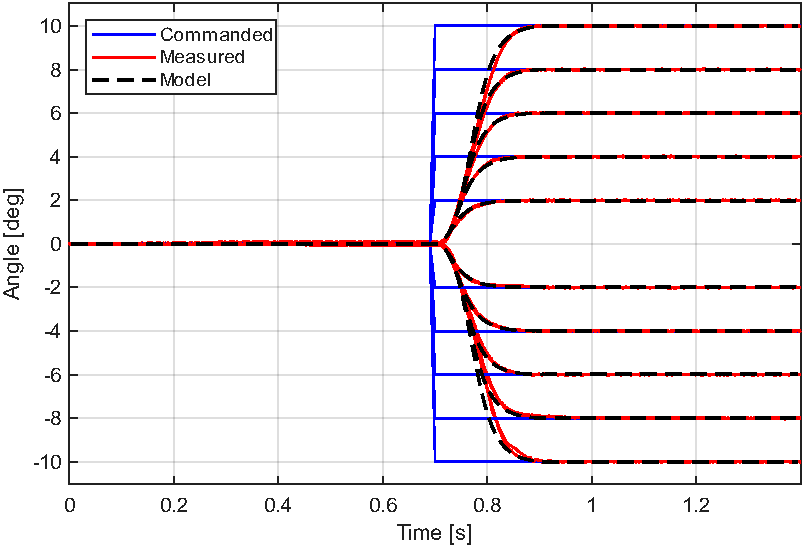
\includegraphics[width=\textwidth]{Figures/stepResponse_canard1.pdf}
        \caption{Ster 1}
        \label{fig:stepresp-canard1}
    \end{subfigure}
    \hfill
    \begin{subfigure}{0.45\linewidth}
        \centering
        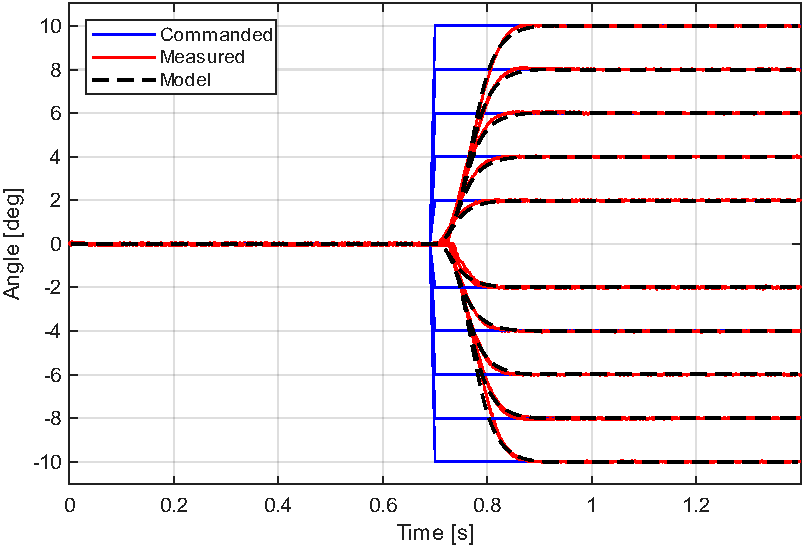
\includegraphics[width=\textwidth]{Figures/stepResponse_canard2.pdf}
        \caption{Ster 2}
        \label{fig:stepresp-canard2}
    \end{subfigure}
    \hfill
    \begin{subfigure}{0.45\linewidth}
        \centering
        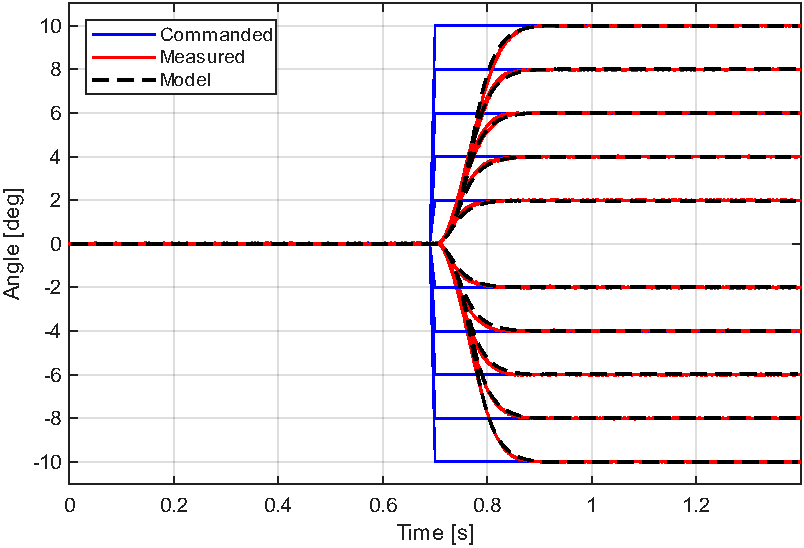
\includegraphics[width=\textwidth]{Figures/stepResponse_canard3.pdf}
        \caption{Ster 3}
        \label{fig:stepresp-canard3}
    \end{subfigure}
    \hfill
    \begin{subfigure}{0.45\linewidth}
        \centering
        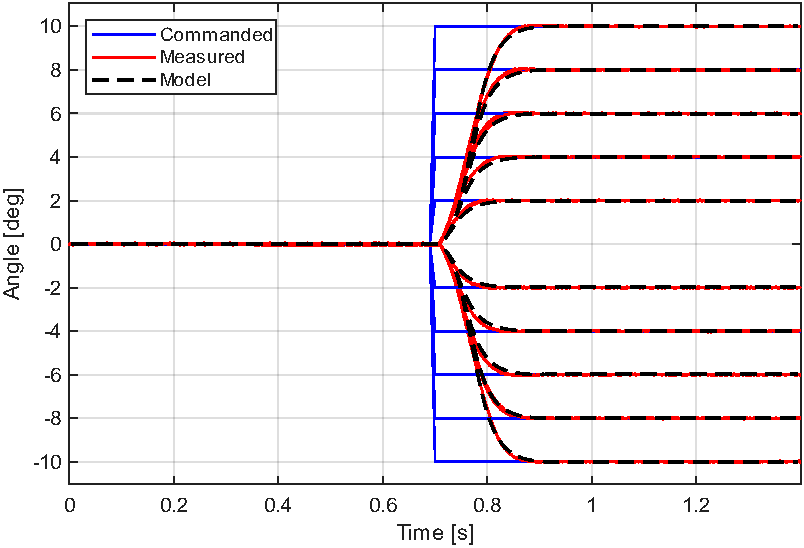
\includegraphics[width=\textwidth]{Figures/stepResponse_canard4.pdf}
        \caption{Ster 4}
        \label{fig:stepresp-canard4}
    \end{subfigure}
    \hfill
    \caption{Porównanie odpowiedzi modelu z rzeczywistą odpowiedzią serw na sygnał skokowy}
    \label{fig:step-resp}
\end{figure}

\begin{table}[H]
    \centering
    \caption{Dobrane parametry modelu serw}
    \label{tab:badania-servo-params}
    \begin{tabular}{lll}
        \hline
        \textbf{Parametr} & Wartość & Jednostka  \\
        \hline
        $\omega_n$ & \num{53.22939340601123}& \unit{\radian\per\s}    \\
        $\zeta$ & \num{1.0160500376693573} & -   \\
        $\epsilon_{\max}$ & \num{59.38028232100888} &  \unit{\radian\per       \s\squared}   \\
        \hline
    \end{tabular}
\end{table}

Oraz przyjęto opóźnienie komunikacyjne \(\tau = \SI{5}{\milli\s}\) co odpowiada jednemu krokowi czasowemu komputera pokładowego rakiety FOK 2D.


\begin{figure}[H]
    \centering
    \begin{subfigure}{0.45\linewidth}
        \centering
        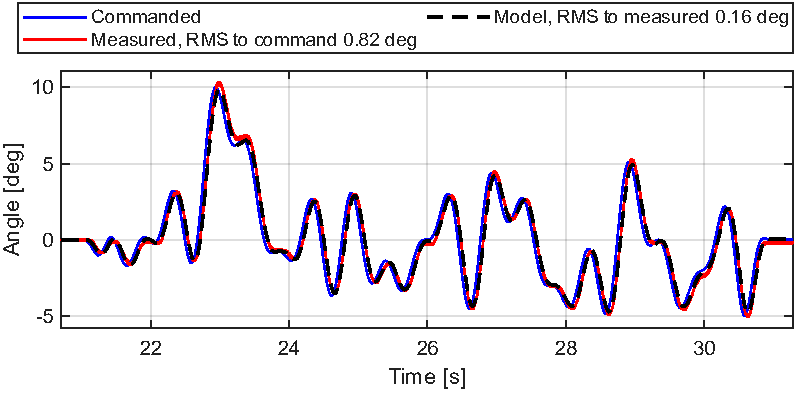
\includegraphics[width=\textwidth]{Figures/validation_canard1_signal1.pdf}
        \caption{Ster 1}
        \label{fig:multisine-canard1}
    \end{subfigure}
    \hfill
    \begin{subfigure}{0.45\linewidth}
        \centering
        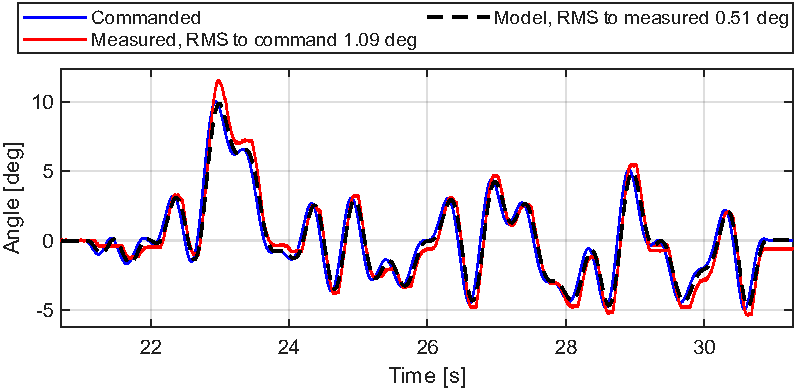
\includegraphics[width=\textwidth]{Figures/validation_canard2_signal1.pdf}
        \caption{Ster 2}
        \label{fig:multisine-canard2}
    \end{subfigure}
    \hfill
    \begin{subfigure}{0.45\linewidth}
        \centering
        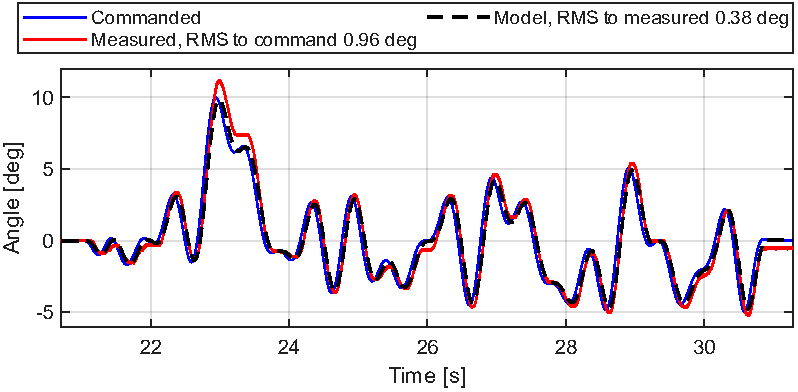
\includegraphics[width=\textwidth]{Figures/validation_canard3_signal1.pdf}
        \caption{Ster 3}
        \label{fig:multisine-canard3}
    \end{subfigure}
    \hfill
    \begin{subfigure}{0.45\linewidth}
        \centering
        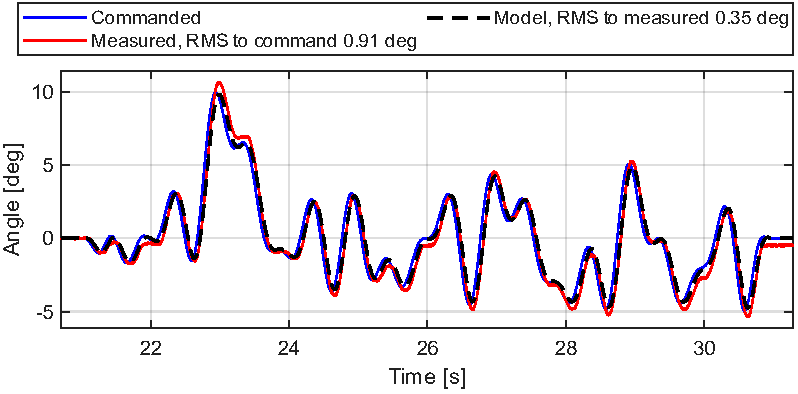
\includegraphics[width=\textwidth]{Figures/validation_canard4_signal1.pdf}
        \caption{Ster 4}
        \label{fig:multisine-canard4}
    \end{subfigure}
    \hfill
    \caption{Porównanie odpowiedzi modelu z rzeczywistą odpowiedzią serw na sygnał wieloczęstotliwościowy}
    \label{fig:multisine}
\end{figure}